
Understanding electron behavior in materials is foundational to modern material science, advancing knowledge of the fundamental properties of matter and simultaneously shaping the development of technologies. The electronic structure and dynamics of materials inform about many of the properties, ranging from conductivity and magnetism to phenomena like superconductivity and topological surface states, making it possible to design new devices and materials with tailored functionalities. These insights allow progress in fields such as semiconductor development, quantum computing, and materials engineering.

We look at an important experimental technique used to study the electronic structure and dynamics: \gls{PES}. The evolution of \gls{PES} has led to several specialized techniques, each offering unique insights into material properties. From conventional \gls{PES} measuring density of states to \gls{ARPES} revealing band structure and many-body effects, to time-resolved variants enabling the study of ultrafast dynamics, these methods have continuously expanded experimental capabilities. The detection of the emitted photoelectrons has similarly evolved, from hemispherical analyzers to the \gls{TOF}-\glspl{MM}, utilizing \glspl{MCP} and \glspl{DLD}. These advanced detection schemes have enabled simultaneous measurement of electron energy, momentum, and temporal information.

As many of the intriguing dynamics such as charge carrier dynamics, phonon interactions \cite{shokeenRealtimeObservationNonequilibrium2024,sjodinUltrafastCarrierDynamics1998,petekFemtosecondTimeresolvedTwophoton1997}, and optically induced phase transitions \cite{laulheUltrafastFormationCharge2017} occur on ultrafast timescales (\unit{fs} to \unit{ps}), the light sources must provide sufficient temporal resolution, i.e.\ sufficiently short pulse durations, to capture these phenomena. \Gls{HHG} and \gls{FEL} sources have become instrumental in this regard, offering the necessary combination of temporal resolution and photon energy tunability. However, these advanced light sources, along with \gls{trPES}, introduce unique challenges. The high photon densities (flux) of these sources can lead to space-charge effects, where Coulomb repulsion between photoemitted electrons distorts their trajectories and energies, distorting measurements and spectral information.

This chapter provides an overview of \gls{PES}, building towards the \gls{MM} instrument--HEXTOF--used to capture the data presented in this thesis\footnote{While there is a dataset we use captured using a different \gls{MM} instrument, it is used for comparison, so the details are not presented.}. Throughout this discussion, we highlight the specific challenges associated with these advanced measurements, particularly those related to space-charge effects, noise, and data quality in \gls{FEL} experiments, motivating the need for the denoising approaches that form the core of this thesis.

\section{Photoemission Process}\label{section:photoemission-process}
In the seminal paper by Einstein \cite{einsteinUberErzeugungUnd1905}, that laid foundations to Quantum Mechanics, Einstein postulated that light is made of discrete quanta of energy $E = h\nu$ to explain the observations by Hertz and J.J. Thompson, explaining the photoelectric effect. The effect can be described as
\begin{equation}\label{eq:photoelectric}
    E_e = h\nu - \phi - |E_B|
\end{equation}
where $E_e$ the emitted kinetic energy, $h$ is the Planck's constant, $\nu$ the frequency of the incoming photon, $\phi$ the material-specific work function and $E_B$ the binding energy referenced to the Fermi level \gls{EF}.

The equation describes how incident photons on a surface emit photoelectrons, provided the photon energy $h\nu$ exceeds $\phi$.
It is then apparent that the binding energy of electrons can be found by irradiating light onto the material and measuring the $E_e$ of photoelectrons. \Gls{PES} is exactly such a technique that leverages this principle to probe the electronic structure of materials.

\cref{eq:photoelectric} also highlights that the kinetic energy of the emitted electrons $E_e$ is dependent on the photon energy but independent of the photon flux (photons per second). However, the flux of photons does affect the number of photoelectrons emitted \cite{foxQuantumOpticsIntroduction2006}. This effect and the probabilistic nature of the photoemission process can be described with the quantum theory of light-matter interaction\footnote{Many of the results can be explained by semi-classical theory as well, which treats the light as a classical wave and the electrons as quantum particles.}.

The whole process of excitation, transport, and emission can be treated as a single coherent process using the formalism of quantum mechanics. This approach incorporates the electronic structure, electron-electron interactions, and the surface barrier in a unified way, and describes the photoemission intensity  $I(E, k_x, k_y)$ being proportional to probability.

The process can be described by the Fermi's Golden Rule, which gives the transition rate between two states. In the context of photoemission, the initial state is the electron in the material, and the final state is the electron in the vacuum. The intensity of photoemission is described by the transition rate between the two states, and the energy conservation:
\begin{equation}
    I(E, k_x, k_y) \propto |\langle \psi_f | \mathbf{A} \cdot \mathbf{p} | \psi_i \rangle|^2 \delta(E - E_f)
\end{equation}
where $\psi_i$ and $\psi_f$ represent the initial and final electron wavefunctions, $\mathbf{A} \cdot \mathbf{p}$ is the matrix element that couples the photon to the electron, and the $\delta$ function ensures energy conservation between the initial and final states.

This highlights the key element that the emission process is a probabilistic event, and hence each event can be described as a random variable. With sufficient observations, the random variables approach their expected value\footnote{This was briefly discussed in the introduction. The reader is also referred to \cref{section:law-of-large-numbers}.}, allowing the material's electronic structure to be resolved. Later in \cref{ch:pes-statistics}, we will discuss the statistical properties of these events in more detail.

In the linear regime, an increase of photon flux results in increased number of photoemitted electrons (or vise versa), but not in $E_e$. However, at high photon fluxes, non-linear photoemission processes start playing a more significant role. In such a case, an electron is emitted after absorbing more than one photon, leading to a deviation from the single-photon flux relation. 

\section{Spectroscopy Techniques}\label{section:spectroscopy-techniques}
A variety of photoemission spectroscopy methods can be devised depending on which parameters are varied and what is measured. Naturally, the most basic setup would measure the energy of the emitted electron as described in \cref{eq:photoelectric}, while variations of the technique allow for additional parameters, such as resolving the electron momentum and spin, or dynamics.

One key technique is \gls{ARPES}, which simultaneously measures the kinetic energy $E_e$ and surface parallel momentum components, \gls{kx} and \gls{ky}, of the emitted electrons, by analyzing their emission angles. By varying the photon energy, \gls{ARPES} can also provide information on the surface perpendicular momentum component \gls{kz}. 

\gls{trPES} takes this process a step further by probing the dynamics of electronic states, allowing to understand transient, non-equibilrium phenomena. A pump-probe scheme is usually employed, where a pump laser drives the system out of equilibrium, and the core- or valence-electron states are probed by a probe laser. By applying a time offset (delay) between the two pulses, the dynamics of the electronic states can be studied as a function of time.

To ensure the statistical significance of time-resolved studies, the repetition rate and flux of the radiation source need to be high enough to capture rare events such as multiphoton processes, to probe excited electronic states with low population densities etc. While \gls{HHG} and \glspl{FEL} sources are well suited for such experiments, having a high flux can be detrimental for \gls{PES} due to the phenomenon known as the \gls{space-charge} \cite{schonhenseMultidimensionalPhotoemissionSpectroscopy2018}.

The space-charge effect occurs when intense light pulses generate a large density electron cloud. This leads to the Coulomb repulsion between electrons, causing a distortion in the electric field, leading to a spread in the energy of the electrons\footnote{Effectively reducing the energy and momentum resolution.}. This effect is more critical in time-resolved studies, as the pump laser creates a pump induced space-charge. To mitigate this, the intensity of the light source must be attenuated, and the most efficient detection schemes must be used in combination with high repetition rate sources.

% In addition to the aforementioned techniques, x-ray photoemission spectroscopy (XPS) focuses on the core-level electrons, providing information on the chemical composition and oxidation states of atoms in a material. By analyzing the binding energies of core electrons, XPS can offer insights into the local electronic environment of atoms. When using hard x-rays for probing, the technique is known as hard x-ray photoelectron spectroscopy (HAXPES).

Measurement of more than three dimensions is generally referred to as \gls{MPES}, such as the simultaneous measurement of energy and all three momentum components. This scheme not only provides a more comprehensive view of the electronic structure but can potentially do so in a short amount of time. Shorter acquisition times help to minimize experimental instabilities, such as beam instability and sample degradation. However, the added dimensions also increase the sample space exponentially, and depend on a correspondingly high flux from the light source to obtain statistically significant data within a reasonable timeframe.

\section{Light Sources}\label{section:light-sources}
As discussed in the previous section, the light source plays a critical role in both \gls{PES} and \gls{trPES}. Other than the necessary high fluence, \gls{XUV} energy and high repetition rate sources are necessary to probe the material, and acquire large amount of data quickly. \gls{trPES} further requires the source to be temporally coherent, with pulse durations on the order of \unit{fs}.

\subsection{High Harmonic Generation}
The most ubiquitous of light sources--the laser--revolutionized experimental science as it enabled a vast range of phenomena to be precisely tested and observed, due to its high spatial and temporal coherence properties. A laser produces its light through a process known as stimulated emission, a process in which electrons, excited to higher energy states by an external energy source, emit photons as they return to lower energy states. These emitted photons, in turn, stimulate other electrons to release additional photons, leading to a cascade of coherent light.

To generate ultrafast, \gls{XUV} light, necessary to probe electronic states in materials, \gls{HHG} is a widely used technique. The \Gls{HHG} principle operates by converting the frequency of \unit{fs} laser pulses into higher harmonic frequencies, resulting in coherent light spanning from extreme ultraviolet to soft x-ray ranges. This is achieved through the non-linear interaction of an intense laser pulse with a gaseous medium, in which electrons are released, accelerated, and then collided with their parent atoms, releasing photons at harmonic multiples of the laser’s original frequency. This approach enables the generation of ultrashort light pulses with energies typically ranging from \qtyrange{10}{100}{eV}, which is well-suited for \gls{trPES} \cite{macklinHighorderHarmonicGeneration1993}. Later in this thesis, we analyze \gls{WSe2} experimental data obtained with a \gls{HHG} source.

\subsection{Free-Electron Laser}\label{section:fel}
Particle accelerators, initially used for high energy physics experiments, which produce radiation as a byproduct of particles accelerating, found their use in spectroscopy. Soon, dedicated facilities providing extremely bright and tunable source of electromagnetic radiation emerged such as Synchrotrons and \glspl{FEL}.
While Synchrotrons are excellent sources of light for a multitude of experiments, they have limitations in terms of the temporal coherence of the light produced. \Glspl{FEL} are linear particle accelerators that produce a pulsed light source with a high temporal coherence, and energies to probe core and deep valence electrons. There are two modes under which \glspl{FEL} operate: \gls{SASE} and seeded.

In \gls{SASE} mode, the amplification process is initiated by the electron shot-noise (\gls{spontaneous_emission}) when the electron beam in the accelerator passes through an undulator. Undulators are periodically arranged magnets that cause the electrons to oscillate and emit radiation. The interaction between the emitted radiation and the charge distribution leads to a phenomenon known as \gls{microbunch} \cite{ackermannOperationFreeelectronLaser2007}. These microbunches emit radiation coherently, leading to the intense, coherent radiation, characteristic of a \gls{FEL}. 

Due to the inherent stochastic nature of the process, the radiation produces intensity fluctuations and hence a lower degree of temporal coherence. Such fluctuations can be seen using a \gls{GMD} (see glossary \gls{gmd} for details) as shown in Figure \ref{fig:gmd-intensity}. The light produced by an \gls{FEL} is of high peak brightness and can be compressed to \unit{fs} pulse durations, making it an ideal source for studying ultrafast phenomena.

To improve the temporal coherence, some \glspl{FEL} such as FERMI \cite{svandrlikDevelopmentPerspectivesFERMI2017} operate in the seeded mode, where a coherent seed laser is used to initiate the amplification process. This leads to a higher degree of temporal coherence in the light produced.

Deutsches Elektronen-Synchrotron DESY is a national research center in Germany that operates the \gls{FLASH} facility \cite{ackermannOperationFreeelectronLaser2007,tiedtkeSoftXrayFreeelectron2009} that produces ultrashort \gls{XUV} and soft X-ray radiation in the wavelength range of \qtyrange{4}{50}{\nm} in the fundamental, and as low as \qty{1.7}{\nm} in the third harmonic, corresponding to a total photon energy range of \qtyrange{25}{830}{\eV}. With an average pulse energy of \qtyrange{1}{500}{\micro\joule}, and pulse durations \qty{<10}{\fs}, peak powers of \qtyrange{1}{5}{\giga\watt} can be reached. This makes it an ideal source for studying ultrafast processes in materials and molecules. An example scheme of the acceleration modules, \glspl{beamline} and experimental end-stations can be seen in Figure \ref{fig:flash-schematic}, where our experiments are performed at the PG2 beamline at FLASH1 (see FLASH1 and 2 in \cref{fig:flash-schematic}).

\begin{figure}
    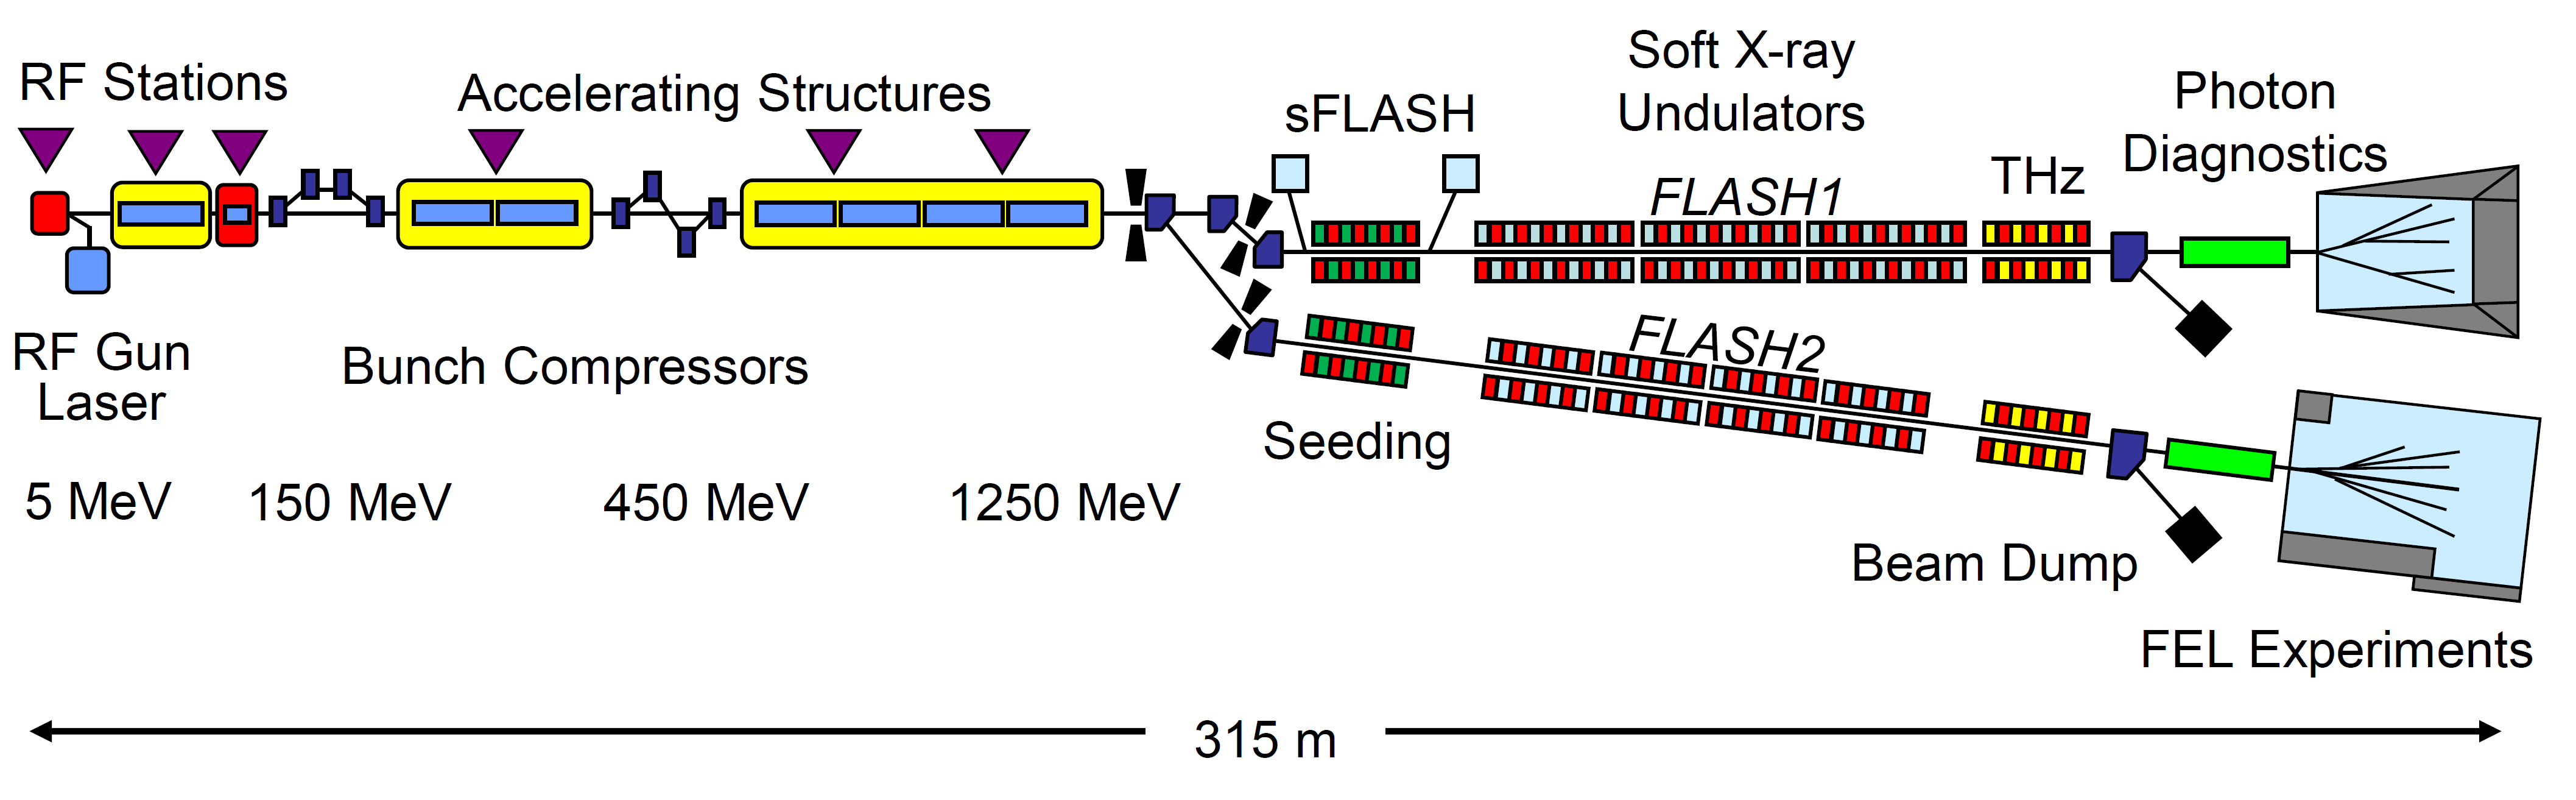
\includegraphics[width=1\linewidth]{images/flash_fel.png}
    \caption{Schematic view of \gls{FLASH}, showing the accelerator section, and the two beamlines: FLASH1 and FLASH2. Reprinted from \cite{faatzSimultaneousOperationTwo2016}, under the terms of the Creative Commons Attribution 3.0 License.}
    \label{fig:flash-schematic}
\end{figure}

As can be seen on the top left of \cref{fig:hex-tof}, \gls{FLASH} provides a very high repetition rate of \qty{1}{\mega\hertz} (or \qty{1}{\micro\second} gap between \glspl{pulse}), but an effective rate of \qty{5}{\kilo\hertz} due to there being \num{500} pulses in each \gls{train}. 

Efficient detection schemes are then necessary to capture all emitted electrons as not only is the repetition rate relatively low, the flux is also attenuated to be below the space-charge limit. Moreover, electron counting detectors typically have a dead-time, meaning that after a measurement, the detector is unable to detect another electron for a certain period of time. This dead-time can be longer than a pulse duration, resulting in the limitation of detecting only a single electron per pulse. Sophisticated detection schemes are then necessary to capture a higher number of emitted electrons, and reduce the acquisition time; the topic of next section.

\section{HEXTOF Instrument}\label{section:hextof}

\begin{figure}
    \centering
    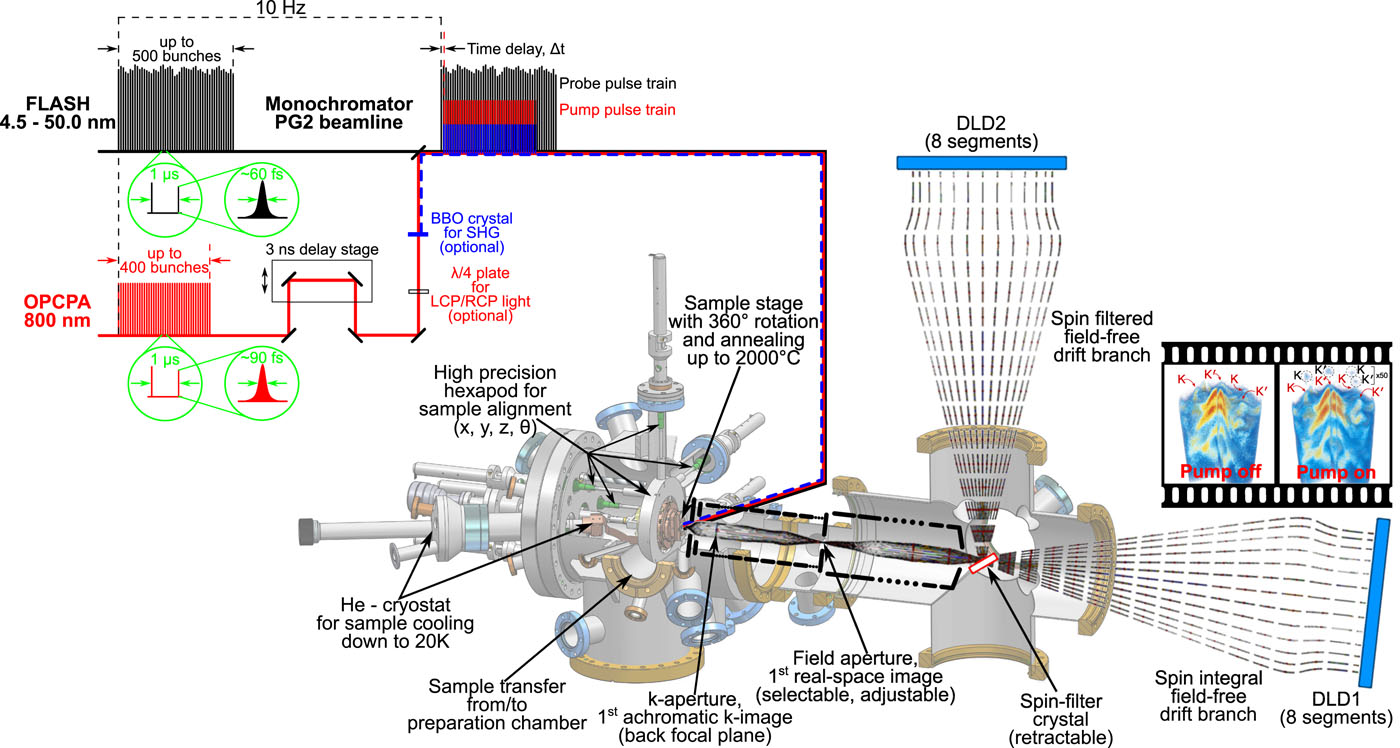
\includegraphics[width=1\linewidth]{images/2024-08-27-10-50-01.png}
    \caption{The simplified overview of the \gls{FLASH} pulse structure, the PG2 beamline with synchronized pump laser (top left) and the \gls{HEXTOF} experimental setup (middle) used to perform time-resolved momentum microscopy.
    Reprinted from \cite{kutnyakhovTimeMomentumresolvedPhotoemission2020}, under the terms of the Creative Commons Attribution 4.0 International License.}
    \label{fig:hex-tof}
\end{figure}

For \gls{PES}, the hemispherical analyzer has long been the preferred instrument, primarily due to its precision in mapping energy-momentum space through an electrostatic lens system and hemispherical energy filter. The analyzer, paired with a 2D detector, can simultaneously measure the energy and azimuthal emission angle, where the emission angle can be mapped to one parallel momentum direction (hence the name \gls{ARPES}). However, it captures only a narrow energy-momentum window at a time, limiting efficiency in high-throughput applications.

More recently, the \gls{MM} with a \gls{TOF}-tube for energy dispersion has been established \cite{schonhenseSpaceTimeSpinresolved2015}. This technique provides a full-field view of the photoemitted electron momentum distribution, offering simultaneous access to the entire momentum space without the need for angular scanning. This, combined with an appropriate detector, provides a 3D data set in energy ($E$) and surface parallel momentum (\gls{kx}, \gls{ky}), enabling efficient acquisition across the entire Brillouin zone\footnote{For a detailed comparison between hemispherical analyzer and \gls{TOF}-\gls{MM}, the reader is referred to \cite{maklarQuantitativeComparisonTimeflight2020}.}. Due to the larger field of view allowing a higher number of photoelectrons to be emitted within each pulse, the space-charge effects can be more pronounced than in hemispherical analyzers.

The \gls{MM} exploits the basic concept from optics where the reciprocal of an image corresponds to its Fourier transform. In the context of \gls{PES}, this means that the reciprocal image of the photoemitted electrons yields, in the back focal plane of a cathode-lens microscope, the projected band structure of the sample under investigation, due to the conservation of parallel momentum in the photoemission process.

The kinetic energies of photoelectrons are resolved through a TOF spectrometer, which consists of a field-free drift tube. In the drift tube, photoelectrons are separated in energy due to their differences in velocity and hit the detector at different times. This setup requires pulsed photon sources, such as the earlier discussed \gls{FEL} and \gls{HHG} sources.

\Glspl{MM} also include a \gls{PEEM} mode, allowing real-space imaging of the sample surface by adjusting the lens system to map the spatial electron distribution instead of momenta. \gls{PEEM} is useful for verifying the spatial overlap of excitation beams and facilitates precise alignment of photon beam positions and focus on the sample. An example of a \gls{PEEM} image can be seen in \cref{fig:chessy-distribution}.

\begin{figure}
    \centering
    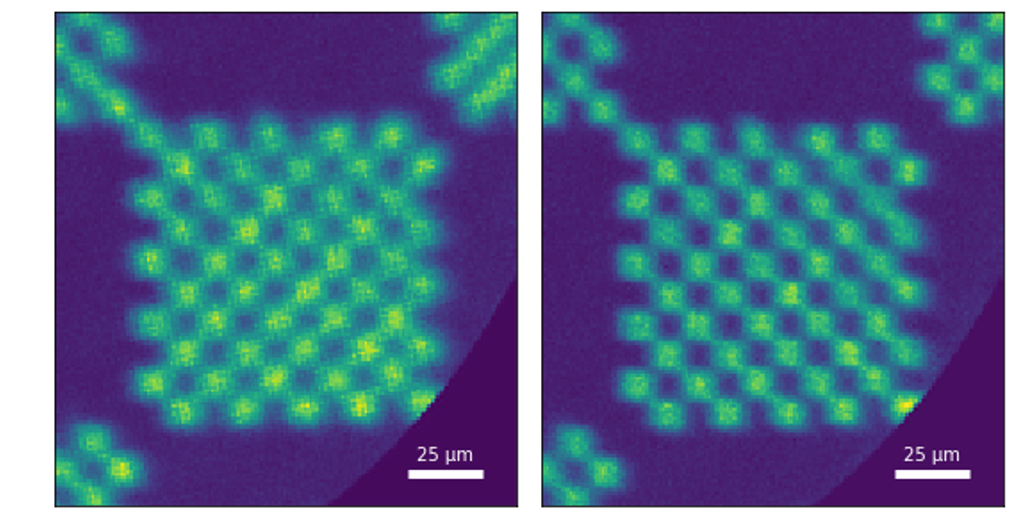
\includegraphics[width=0.7\linewidth]{images/chessy_deblurring_merged_events.png}
    \caption{Chessy sample before and after merging double-counted events, showing better resolved features. Chessy test sample is employed to determine the spatial overlap and field of view alignment in a momentum microscope using the \gls{PEEM} mode. Courtesy of M. Heber.}
    \label{fig:chessy-distribution}
\end{figure}

The \gls{HEXTOF} instrument \cite{kutnyakhovTimeMomentumresolvedPhotoemission2020}, shown in \cref{fig:hex-tof}, is based on this \gls{TOF}-\gls{MM} scheme to perform core- and valence-electron time- and momentum-resolved studies at \gls{FLASH}, utilizing a specialized \num{8}S-\gls{DLD} for capturing electron distributions, discussed in the next section. This instrument captured majority of the data presented in this thesis, with the exception of \gls{WSe2} data, captured using another \gls{MM} instrument in combination with a \gls{HHG} source \cite{maklarQuantitativeComparisonTimeflight2020}.

One of the standout features of \gls{HEXTOF} is its multidimensional recording scheme. This approach allows for simultaneous measurement of multiple parameters that can be related to the complete momentum space \gls{kx}, \gls{ky}, \gls{kz}, energy \gls{E}, and delay time \gls{tpp}. The \gls{kx} and \gls{ky} are recorded based on the direction of the emitted electrons, while the \gls{kz} is determined by tuning the photon source. The \gls{E} is determined by the time-of-flight of the electrons, and the \gls{tpp} is the delay between the pump and probe pulses. More recently, the spin branch has been explored and spin polarization added to the list of parameters that can be measured. 

\section{Delay Line Detector}\label{section:dld}
\subsection{Microchannel Plate}
Individual electrons released by the photoemission process are difficult to directly detect due to their small charge.  Therefore, it is necessary to have an amplification process to allow their detection. \Gls{MCP} is one such amplifier, that is sensitive to electrons\footnote{\Glspl{MCP} are versatile as they are also sensitive to high energy photons in the \gls{XUV} regime, and also to charged particles.}

\begin{figure}[h]
    \centering
    \begin{subfigure}[t]{0.49\linewidth}
        \centering
        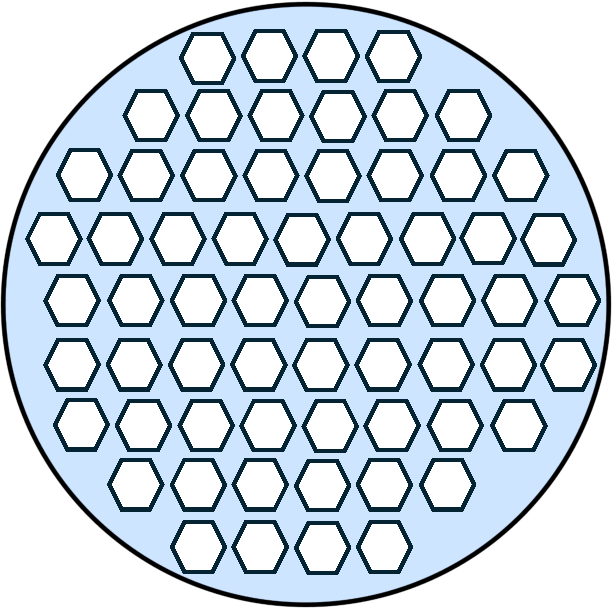
\includegraphics[width=\linewidth]{images/mcp.pdf}
        \caption{Illustrative front view of a circular \gls{MCP} showing an enlarged hexagonal microchannel structure. \Glspl{MCP} contain millions of such microchannels packed at a microscopic scale, each capable of amplifying electron cascades.}
        \label{fig:mcp}
    \end{subfigure}
    \hfill
    \begin{subfigure}[t]{0.49\linewidth}
        \centering
        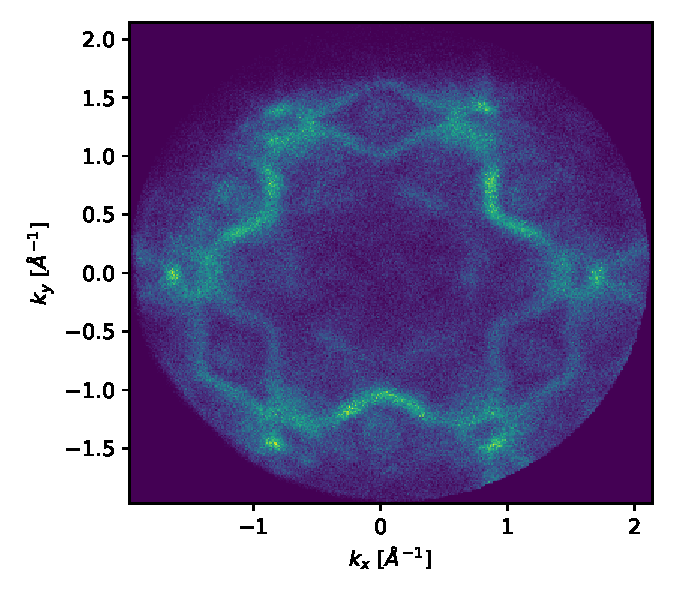
\includegraphics[width=\linewidth]{images/calibrated_momentum.pdf}
        \caption{Calibrated \gls{kx}--\gls{ky} map of \gls{GrIr} near \gls{EF}. This map represents the momentum distribution of photoelectrons detected by the \gls{HEXTOF} setup, with pixel values mapped to physical momentum axes.}
        \label{fig:grir-2d-slice-calibrated}
    \end{subfigure}
    \caption{(a) Illustrative view of the circular \gls{MCP}, showing its hexagonal microchannel structure, which plays a critical role in amplifying electron signals within the detection system. (b) Circular momentum map of the \gls{GrIr} dataset in the \gls{kx}--\gls{ky} plane, derived from measurements using the full detection setup, which includes the \gls{MCP} as part of the \gls{TOF}-\gls{MM} and \gls{DLD} configuration. Both the MCP structure and momentum map share a circular geometry, reflecting the consistent spatial organization across the detection system.}
    \label{fig:combined-figures}
\end{figure}

\Glspl{MCP} are structured dense 2D array of hexagonal microchannels (with \unit{\micro\meter} sizes), as can be seen in \cref{fig:mcp}. With millions of such channels, each charge cloud can be localized. When an electron strikes the surface of the \gls{MCP}, it generates a cascade of secondary electrons, resulting in a final charge cloud that is orders of magnitude stronger than the initial signal. For additional gain, the \glspl{MCP} can be stacked in two layers, with V-stack (Chevron) configuration\footnote{Alternate configuration with an even higher gain by stacking together three layers is known as Z-stack.}
as can be seen in top of \cref{fig:dld}, where the V shape is visible when viewing MCP 1 and MCP 2 together \cite{ladislaswizaMicrochannelPlateDetectors1979,paschottaMicrochannelPlatesEncyclopedia2019}. 

The amplified charge cloud is then collected by a readout system, such as  phosphor screens paired with a \gls{CCD}, resistive anodes, wedge-and-strip anodes, and pixelated detectors. In the phosphor screen method, phosphor screen that converts the charge cloud into light, which can be detected by, e.g., a \gls{CCD} camera. The phosphor--\gls{CCD} scheme provides a high spatial resolution of the electrons to be recorded, but lacks the temporal resolution necessary for \gls{trPES}, i.e., it has a much slower decay time than the dynamics being studied.

Pixelated detectors, which divide the anode into discrete segments, provide an alternative means to capture spatial information with high precision. However, the need to read each pixel individually limits their processing speed, as each pixel must be sequentially analyzed. While this approach supports multiple simultaneous hits across the pixel grid, it remains inadequate for experiments requiring rapid data acquisition and precise temporal resolution. Improvements in the readout speed have been suggested and the prospect of using pixelated detectors in future experiments is being realized \cite{correaTEMPUSTimepix4basedSystem2024}.

\subsection{MCP with Delay-line readout}
\begin{figure}
    \centering
    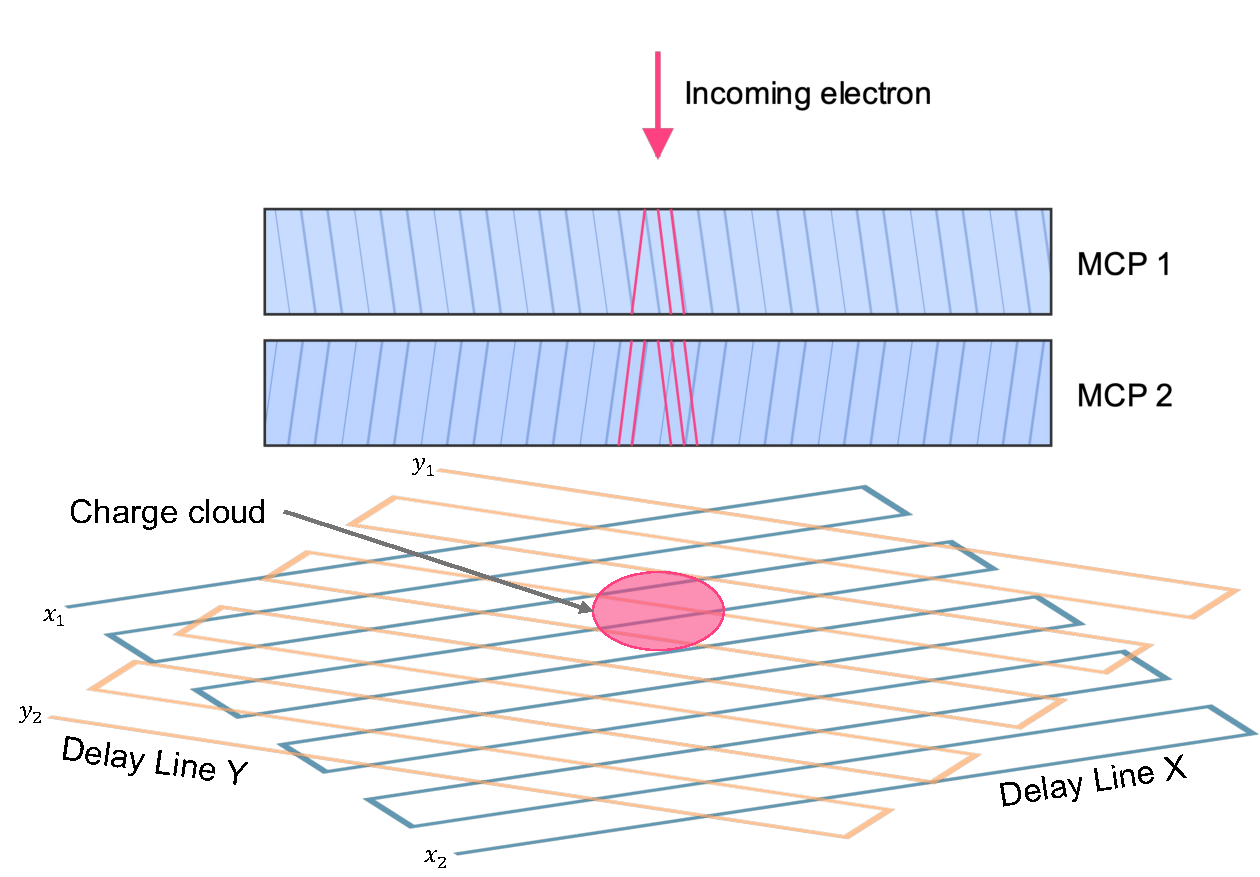
\includegraphics[width=0.9\linewidth]{images/dld.pdf}
    \caption{Diagram of an example \gls{DLD}, with an \gls{MCP} and a delayline structure. \textbf{\gls{MCP} Structure}: The \glspl{MCP} are arranged in a V-stack (Chevron) configuration, with microchannels at opposite tilt angles to enhance electron cascade efficiency. Each channel, shown as simplified lines within the semi-transparent blue \gls{MCP} layers, initiates an electron cascade upon impact. This cascade amplifies the signal across both \glspl{MCP}, preserving spatial information and forming a final charge cloud. \textbf{Delayline Structure}: Below the \glspl{MCP}, the $x$ and $y$ meandering delay lines are presented, rotated \qty{45}{degree} relative to one another, illustrating how each delay line (labeled X and Y) captures spatial information through the timing of signals between designated endpoints ($x_1$, $x_2$, $y_1$, $y_2$).}
    \label{fig:dld}
\end{figure}
\Glspl{MCP} in combination with a delay-line readout are known as \glspl{DLD} \cite{oelsnerMicrospectroscopyImagingUsing2001}. \Glspl{DLD} have the unique ability to capture single-event data with high spatiotemporal accuracy. As shown in \cref{fig:dld}, a delay-line readout includes two orthogonal meandering\footnote{This zigzag pattern increases effective length, allowing for finer temporal resolution and hence position.} delay lines (meanders), positioned beneath the MCP, labeled Delay Line X and Y. When an electron strikes the \gls{MCP}, the resulting amplified charge cloud is transmitted to the delay lines. The charge propagates in both directions along each delay line, with timing recorded at each endpoint ($x_1$, $x_2$, $y_1$, $y_2$) by a time-to-digital converter (TDC). By calculating timing differences along the $x$ and $y$ axes, the exact position of the electron impact is determined and by using a reference trigger, the arrival time of the electron $t_{\text{tof}}$ can also be determined. This allows precise determination of the electron's position in both \gls{PEEM} and \gls{MM} modes, providing real and surface parallel momentum information, respectively.

The \gls{DLD} is also able to record the electron \gls{TOF}, which is synchronized to the photon pulse source. The \gls{TOF} can be measured by recording the initiation of the event (when the photon pulse comes) till when they hit the meanders. Since electrons with different energies travel at different velocities, the \gls{TOF} can be used to determine the kinetic energy of the electrons.

The issue with these detectors is that the meanders experience a dead-time on the \unit{ns} scale after each event. This allows only some collected electrons to be detected, necessitating a higher acquisition time. An alternative to this is segmenting the detector. One way is to add more 2D meanders and assign them to different sections of the \gls{MCP} (with overlaps to have no missing location), such as having the meanders in different quadrants of the \gls{MCP}. This allows for the detection of multiple electrons simultaneously. Another is to layer these meanders vertically behind each other, as the meander experiencing dead-time is mostly invisible to the electrons, and the next layer can detect the electrons. Stacking up to \num{128} meander layers is currently under development \cite{oelsnerTimeEnergyResolved2010}.

\subsection{HEXTOF 8S-DLD}\label{section:8s-dld}
The detector used in the \gls{HEXTOF} instrument uses a combination of these approaches, with a 2-layer, 4-quadrant structure, known as the 8S-DLD. The 8S-DLD is hence capable of detecting multiple electrons simultaneously, providing a more comprehensive view of the photoelectron distribution. However, the multi-layer detection scheme comes with a caveat: when an electron cloud strikes in locations where two quadrants meet\footnote{This is always the case for 2 or more layered schemes.}, special adjustments need to be made to not detect the event twice. To that end, layers must be appropriately calibrated otherwise the electron counting routines can report multiple events for the same electron, reporting different momentum and energy values for the same electron event. 

With a correlation analysis on the photoelectrons generated in pulses, this effect has been observed by \citeauthor{heberStudiesUltrafastDynamics2024} \cite{heberStudiesUltrafastDynamics2024}. This effect not only wrongly counts electrons but also distorts (blurs) the momentum distribution. \citeauthor{heberStudiesUltrafastDynamics2024} further demonstrates that by first finding the multi-counted events and averaging them, the resolution of \gls{MM} can be improved as can be seen on the right of \cref{fig:chessy-distribution}, compared to the distorted distribution on the left.

For the interested reader, we also point to the work by \citeauthor{knipferDeepLearningbasedSpatiotemporal2024} who have proposed a deep learning based method to reconstruct the events accurately \cite{knipferDeepLearningbasedSpatiotemporal2024}, significantly improving reconstruction done by prior \gls{DLD} codes.